\documentclass{article}
\usepackage{amsmath}
\usepackage{amssymb}
\usepackage{graphicx}
\usepackage{float}
\usepackage{booktabs}
\usepackage{geometry}
\usepackage{listings}
\usepackage{xcolor}

\geometry{margin=2.5cm}

\title{\textbf{Report on Inverse Modelling Exercise}\\

\large DA7067 Computational Mathematics}

\author{ Onyinyechi Sonia Bäckström, Christoffer Janson, Yuqi Yang \\
Stockholm University}

\date{September 2026}

\begin{document}

\maketitle
\newpage
\section{Introduction}
The aim of this exercise is to construct an inverse model for an ice
sheet and use observed surface height and horizontal velocity data to
estimate the underlying bedrock geometry.

The bedrock is assumed to consist of a base slope with two Gaussian-like
bumps. The locations and shapes of the two bumps are known, while their
amplitudes are unknown. Therefore, the inverse problem is to determine
the two bump amplitudes from the available surface observations.

The exercise also investigates the effect of measurement noise. A small
amount of random noise is added to the surface height and horizontal
velocity data, and the inverse calculation is repeated to determine how
the estimated bedrock amplitudes are affected.

The inverse calculation does not use the transient free-surface equation,
because the observation time is unknown. Instead, the observed surface
height and velocity are used directly to reconstruct the ice thickness
and bedrock.
\section{Ice Sheet Model}

The supplied model uses the shallow ice approximation (SIA). The
parameters used in the forward model are

\begin{equation}
L = 10^5,
\end{equation}

\begin{equation}
A = 300,
\end{equation}

\begin{equation}
\rho = 9.138\times10^{-19},
\end{equation}

\begin{equation}
g = 9.7692\times10^{15},
\end{equation}

and

\begin{equation}
n=3.
\end{equation}

The ice sheet domain is divided into $51$ grid points. The initial ice
thickness is $800$ m and the bedrock has a base slope determined by an
angle of $0.2^\circ$.

The bedrock is represented by a sloping base with two Gaussian-shaped
bumps. The supplied function \texttt{CreateBedRock} constructs the
bedrock according to

\begin{equation}
b(x) = b_{\mathrm{base}}(x)
       +a_1B_1(x)
       +a_2B_2(x),
\end{equation}

where $a_1$ and $a_2$ are the two unknown amplitudes and $B_1$ and
$B_2$ are the two prescribed bump functions.

The base bedrock is

\begin{equation}
b_{\mathrm{base}}(x)=-\tan(\theta)x,
\end{equation}

where $\theta=0.2^\circ$.

The two bump positions are fixed by the supplied model. Therefore, the
inverse problem only needs to determine the two amplitudes $a_1$ and
$a_2$.


\section{Inverse Modelling Method}

The inverse calculation uses the observed surface elevation $h$ and
horizontal velocity $u_x$.

The transient free-surface equation is not used in the inverse
calculation because the observation time is unknown. Instead, the
observed surface and velocity are used directly to reconstruct the
ice thickness and bedrock.

\subsection{Calculation of the Surface Gradient}

The first step is to calculate the surface gradient

\begin{equation}
\frac{dh}{dx}.
\end{equation}

The gradient is calculated using finite differences. For an interior
grid point, the central difference is

\begin{equation}
\frac{dh}{dx}
\approx
\frac{h_{j+1}-h_{j-1}}{2\Delta x}.
\end{equation}

 The calculated surface gradient is shown in Figure ~\ref{fig:surfgrad}.
This gradient is used in the velocity relation to estimate the ice thickness. 
\\
\begin{figure}[H]
    \centering
    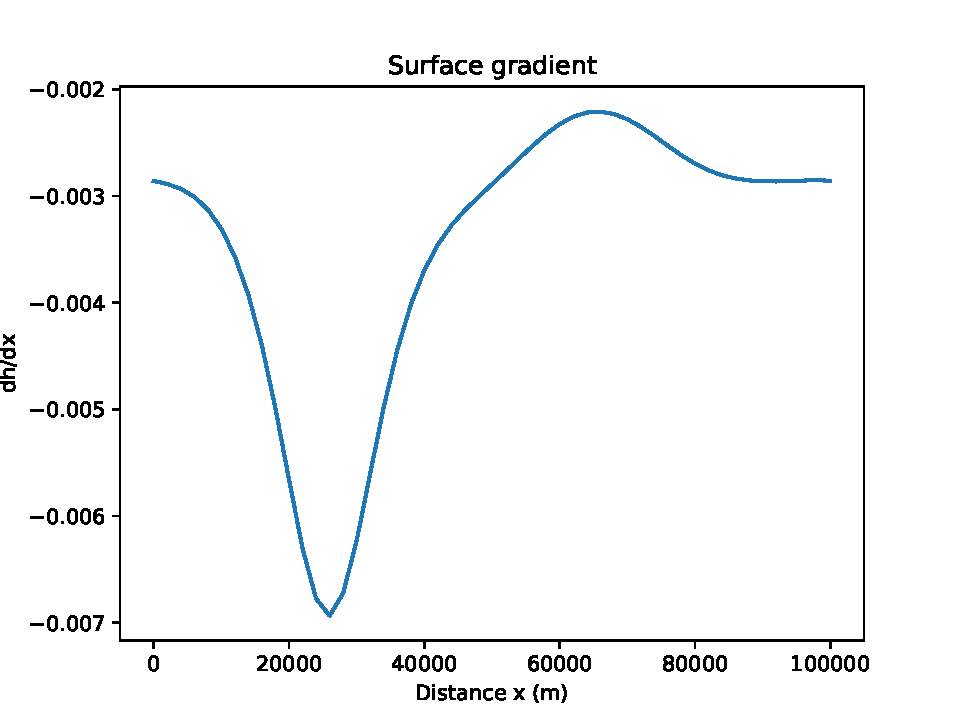
\includegraphics[width=0.8\linewidth]{plots/surfacegradient.pdf}
    \caption{the surface gradient}
    \label{fig:surfgrad}
\end{figure}

\subsection{Calculation of Ice Thickness}

The horizontal velocity relation used in the inverse model was taken
directly from the supplied \texttt{icemodel.py}. The model calculates
the horizontal velocity according to

\begin{equation}
u_x =
-\frac{2A(\rho g)^n}{n+1}
\left(\frac{dh}{dx}\right)^n
H^{n+1},
\end{equation}

where $H$ is the ice thickness.

Since the surface velocity and surface elevation are available from the
observations, while the ice thickness is unknown, this equation can be
rearranged to calculate $H$.

Multiplying by $(n+1)$ gives

\begin{equation}
u_x(n+1)
=
-2A(\rho g)^n
\left(\frac{dh}{dx}\right)^n
H^{n+1}.
\end{equation}

Therefore,

\begin{equation}
H^{n+1}
=
\frac{u_x(n+1)}
{-2A(\rho g)^n
\left(\frac{dh}{dx}\right)^n}.
\end{equation}

Taking the power $1/(n+1)$ gives

\begin{equation}
\boxed{
H =
\left[
\frac{u_x(n+1)}
{-2A(\rho g)^n
\left(\frac{dh}{dx}\right)^n}
\right]^{1/(n+1)}
}.
\end{equation}
The result is shown in figure \ref{fig:icethick}.
\begin{figure}[H]
    \centering
    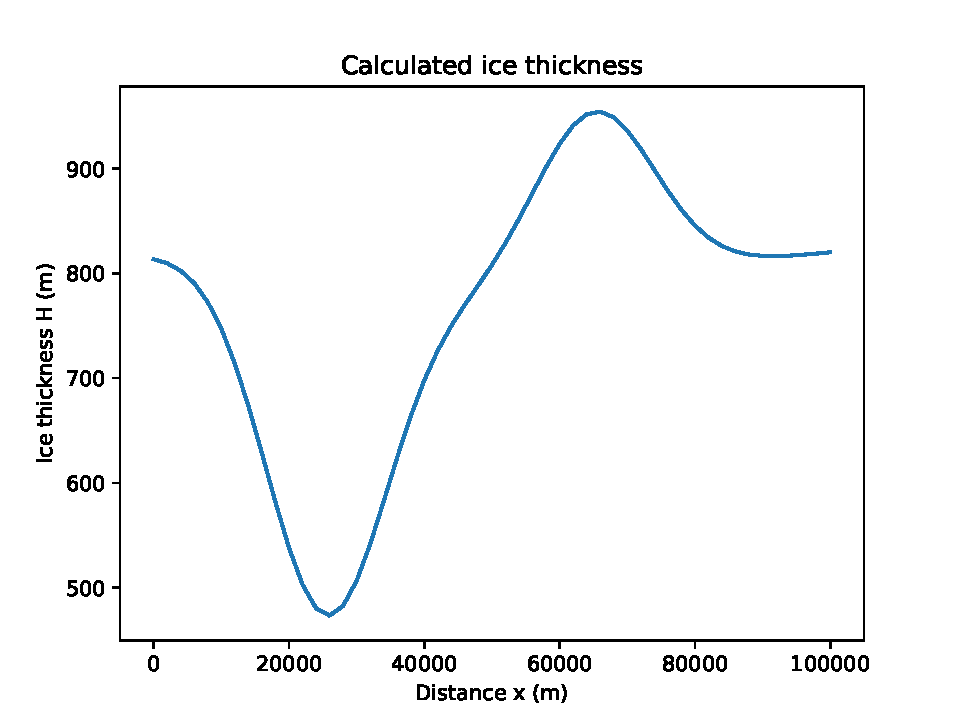
\includegraphics[width=0.8\linewidth]{plots/calculatedicethickness.pdf}
    \caption{the ice thickness}
    \label{fig:icethick}
\end{figure}
 Where the ice thickness is thinner the bedrock should have a similar increase in height and where the ice is thicker the bedrock should be lower.
\subsection{Calculation of Bedrock}

Once the ice thickness has been calculated, the bedrock elevation can
be reconstructed from the relationship

\begin{equation}
\boxed{b = h-H}.
\end{equation}

Using the observations, the reconstructed ice thickness was found to
range approximately from

\begin{equation}
473.3\ \mathrm{m}
\leq H
\leq
954.5\ \mathrm{m}.
\end{equation}

This range is reasonable for an ice sheet with a nominal thickness of
approximately $800$ m.
 The results are shown in figure \ref{fig:reconbedrock}.
\begin{figure}[H]
    \centering
    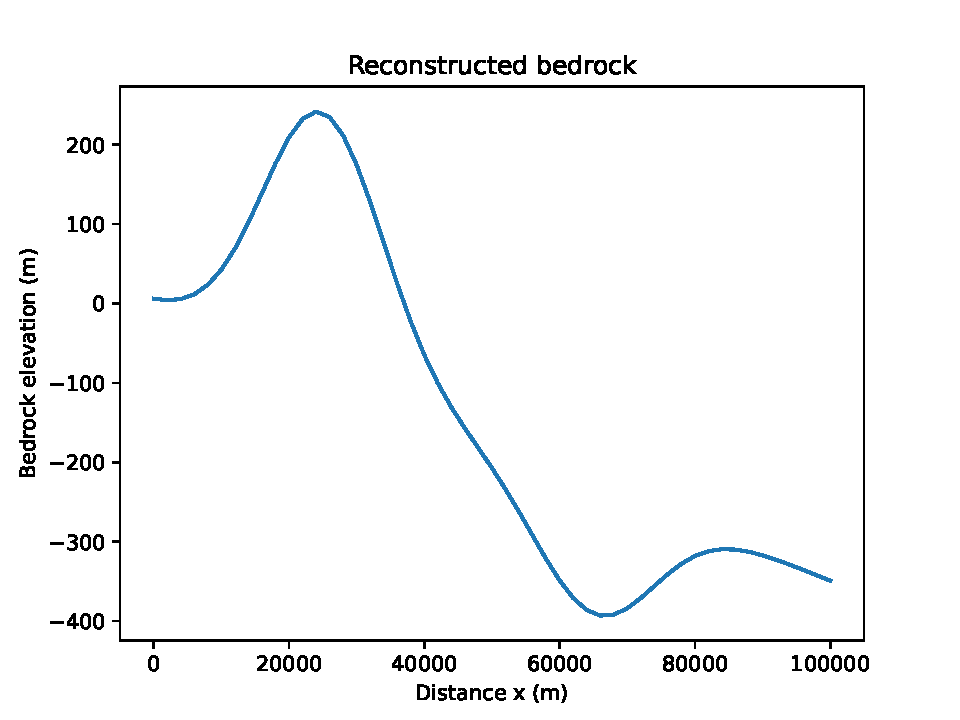
\includegraphics[width=0.8\linewidth]{plots/reconstructedbedrock.pdf}
    \caption{the reconstructed bedrock}
    \label{fig:reconbedrock}
\end{figure}
\begin{figure}[H]
    \centering
    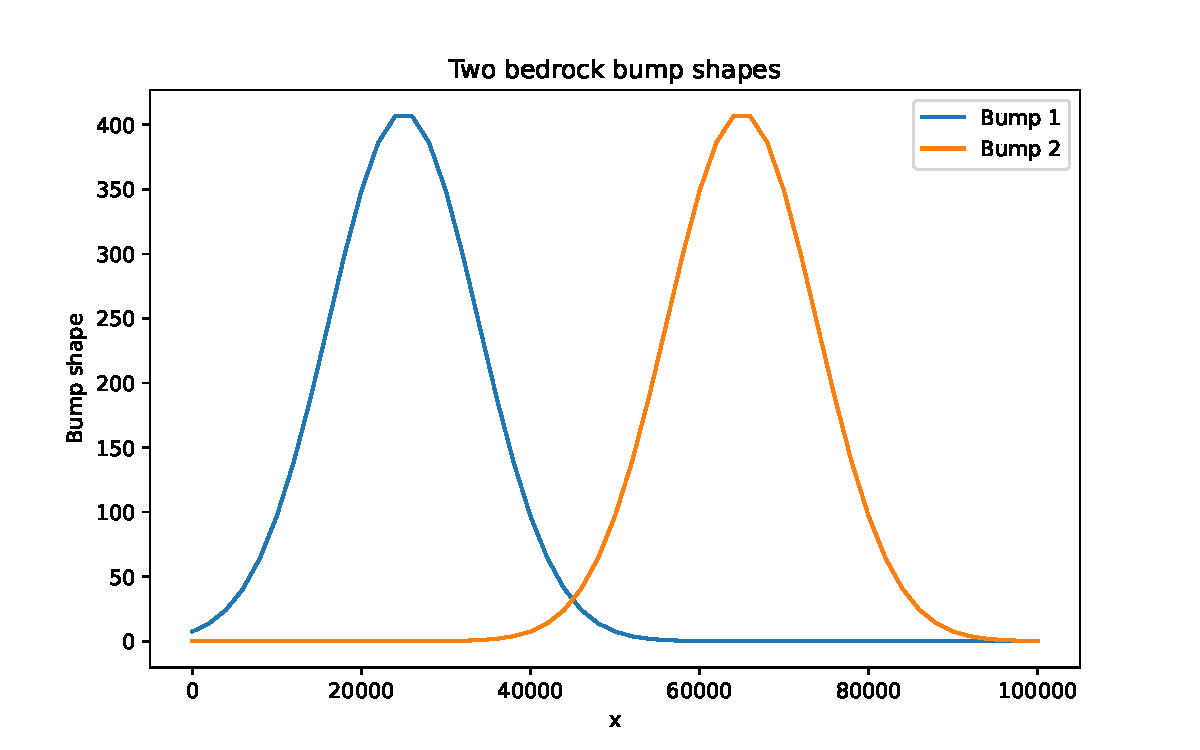
\includegraphics[width=0.8\linewidth]{plots/bumpshape.pdf}
    \caption{the bumps}
    \label{fig:bumps}
\end{figure}

\section{Determination of Bedrock Amplitudes}

The reconstructed bedrock is fitted using the two-bump bedrock model
from the supplied \texttt{icemodel.py}.

The model can be written as

\begin{equation}
b(x)
=
b_{\mathrm{base}}(x)
+a_1B_1(x)
+a_2B_2(x).
\end{equation}

The reconstructed bedrock is therefore compared with the model
prediction, and the unknown amplitudes are found using a least-squares
fit.

The resulting amplitudes are

\begin{equation}
\boxed{a_1 \approx 0.8000},
\end{equation}

and

\begin{equation}
\boxed{a_2 \approx -0.4000}.
\end{equation}

The fitted bedrock is

\begin{equation}
b_{\mathrm{fit}}(x)
=
b_{\mathrm{base}}(x)
+0.8B_1(x)
-0.4B_2(x).
\end{equation}

These amplitudes were chosen because they gave the best least-squares fit between the two-bump bedrock model and the reconstructed bedrock.

\begin{table}[H]
\centering
\caption{Estimated bedrock amplitudes from the inverse model.}
\label{tab:amplitudes}
\begin{tabular}{ccc}
\toprule
Parameter & Estimated value & Method \\
\midrule
$a_1$ & $0.8000$ & Least-squares fit \\
$a_2$ & $-0.4000$ & Least-squares fit \\
\bottomrule
\end{tabular}
\end{table}
\begin{figure}[H]
    \centering
    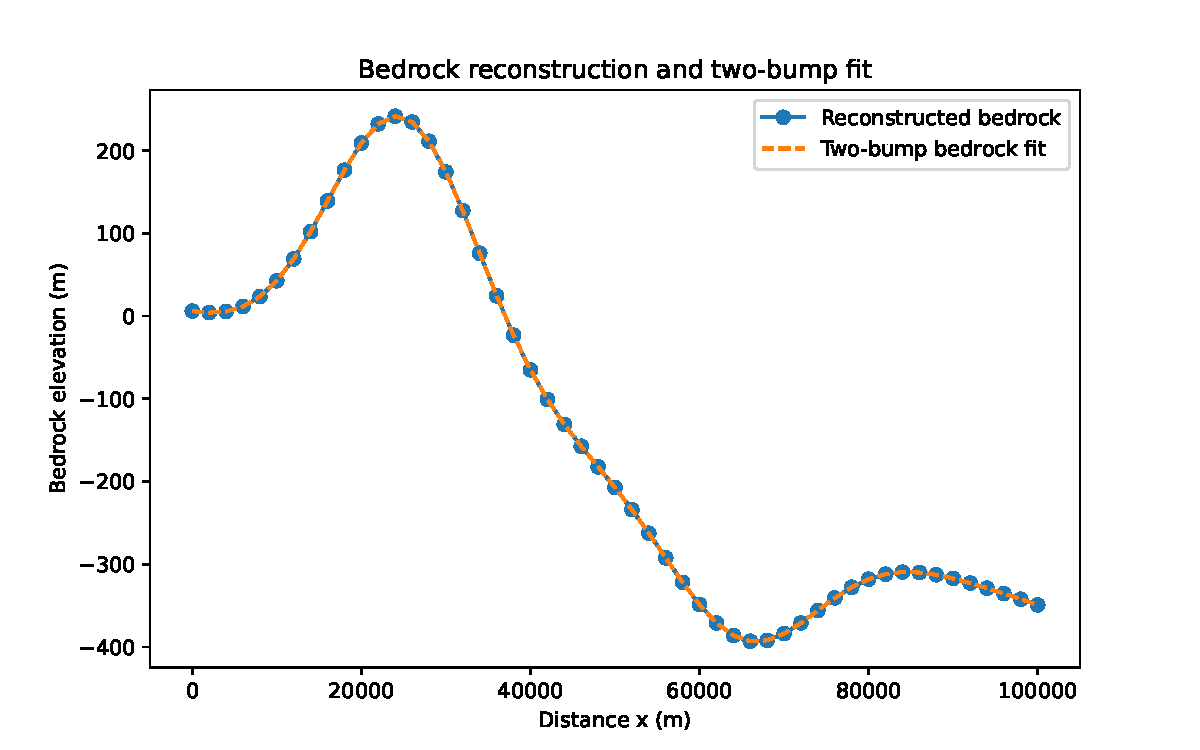
\includegraphics[width=0.8\linewidth]{plots/bedrockandtwobumpfit.pdf}
    \caption{the bumps and reconstructed bedrock fitted using $a_1=0.8$ and $a_2=-0.4$.}
    \label{fig:bedrockbumpfit}
\end{figure}


\section{Forward Model Verification}

The estimated bedrock amplitudes were then used as input to the forward
model. The purpose of this simulation was to demonstrate the evolution of the ice sheet when the bedrock obtained from the inverse
model is used as input.

The amplitudes used in the forward simulation were

\begin{equation}
a_1=0.8,
\qquad
a_2=-0.4.
\end{equation}

The forward model was run for 200 years using the inferred bedrock.
The surface was updated using the velocity and surface-gradient
calculation supplied in the model.

The resulting surface elevation and bedrock are shown in figure \ref{fig:forward200}.
\begin{figure}[H]
    \centering
    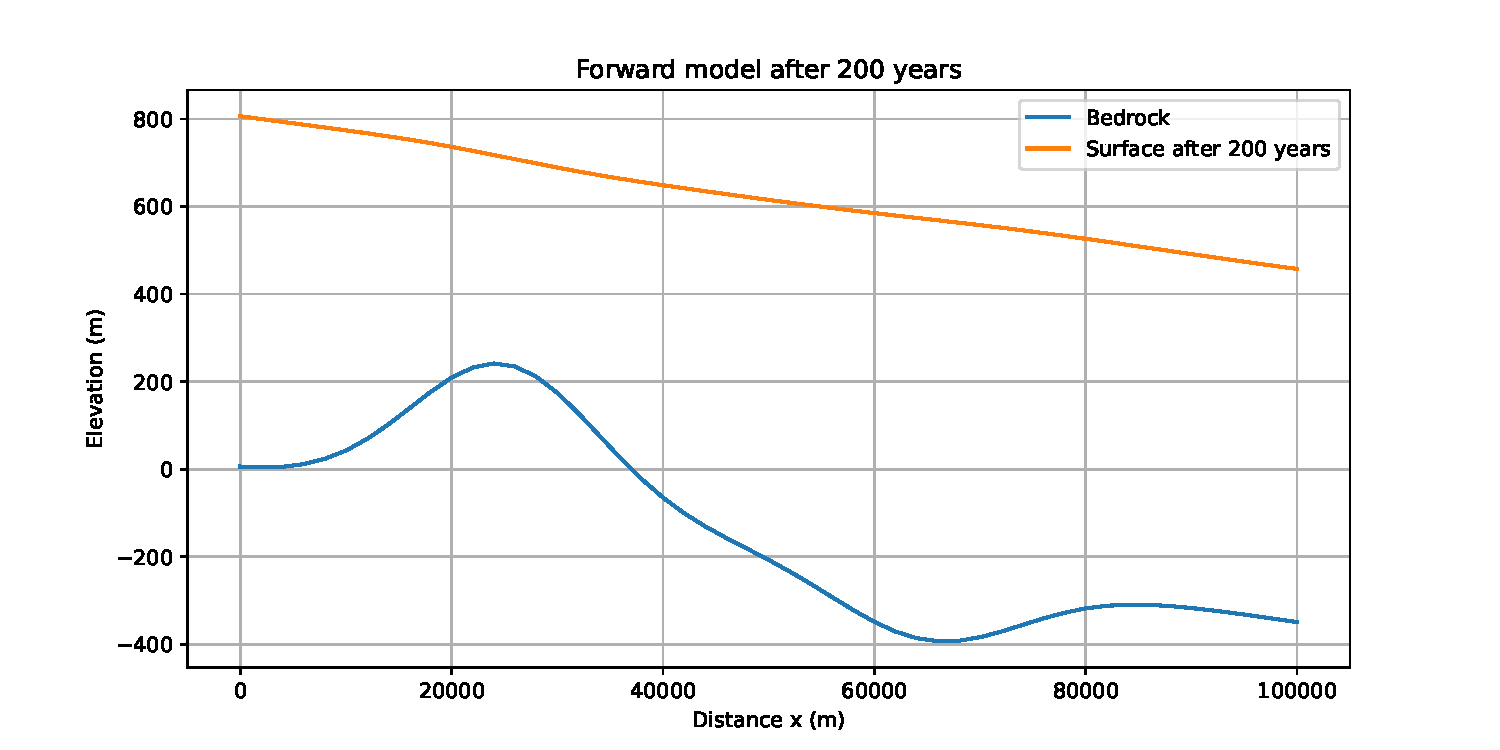
\includegraphics[width=0.8\linewidth]{plots/forwardmodel200years.pdf}
    \caption{the resulting amplitudes used with the forward model to simulate 200 years of glacial movment}
    \label{fig:forward200}
\end{figure}

\subsection{Effect of Random Noise}

To investigate the sensitivity of the inverse model to measurement
noise, random noise was added to both the observed surface elevation
$h$ and the horizontal velocity $u_x$. The same direct inversion method
used for the noise-free data was applied at each noise level. Therefore,
the inverse method was kept unchanged and only the magnitude of the
measurement noise was varied.

Noise levels of $0\%$, $1\%$, $2\%$, $5\%$, and $10\%$ were considered.
The same random noise pattern was used for all noise levels, with its
magnitude scaled according to the specified noise level. This allows
the effect of increasing noise to be compared more consistently.

For each noise level, the noisy surface gradient was calculated using
finite differences. The ice thickness was then calculated from the
horizontal velocity relation,

\begin{equation}
H =
\left[
\frac{u_x(n+1)}
{-2A(\rho g)^n
\left(\frac{dh}{dx}\right)^n}
\right]^{1/(n+1)},
\end{equation}

and the bedrock was reconstructed using

\begin{equation}
b=h-H.
\end{equation}

The same least-squares fitting procedure was then used to estimate the
two bedrock amplitudes.

\begin{table}[H]
\centering
\caption{Estimated bedrock amplitudes for different noise levels.}
\label{tab:noise_results}
\begin{tabular}{ccc}
\toprule
Noise level & $a_1$ & $a_2$ \\
\midrule
$0\%$  & 0.8000 & -0.4000 \\
$1\%$  & 0.1953 & -0.4932 \\
$2\%$  & 0.6118 & -0.5201 \\
$5\%$  & 1.5751 & 0.8293 \\
$10\%$ & 1.6844 & 1.3866 \\
\bottomrule
\end{tabular}
\end{table}


Random noise makes it more difficult to determine the bedrock amplitudes
accurately. This is because noise in the observed surface elevation and
horizontal velocity affects the calculated surface gradient and ice
thickness. As a result, the reconstructed bedrock becomes less accurate,
which affects the estimated amplitudes $a_1$ and $a_2$.

For the noise-free data, the estimated amplitudes were
$a_1=0.8$ and $a_2=-0.4$. When 2\% random noise was added, the
estimated amplitudes changed to approximately $a_1=0.612$ and
$a_2=-0.520$. At higher noise levels, the difference becomes more pronounced. At
$5\%$ noise, the estimated amplitudes are $a_1=1.5751$ and
$a_2=0.8293$, while at $10\%$ noise they become $a_1=1.6844$ and $a_2=1.3866$. In particular, the estimated value of $a_2$ changes sign between $2\%$ and $5\%$ noise.This shows that measurement noise can change the estimated
bedrock amplitudes and therefore reduces the accuracy with which the
bedrock can be determined.

The relationship is not monotonic, meaning that the estimated amplitudes do not simply increase or decrease as the noise level increases. However, the estimates become increasingly different from
the noise-free values at higher noise levels. These results indicate that the direct inverse calculation is sensitive to measurement noise,
which reduces the accuracy with which the bedrock amplitudes can be determined.
\begin{figure}[H]
    \centering
    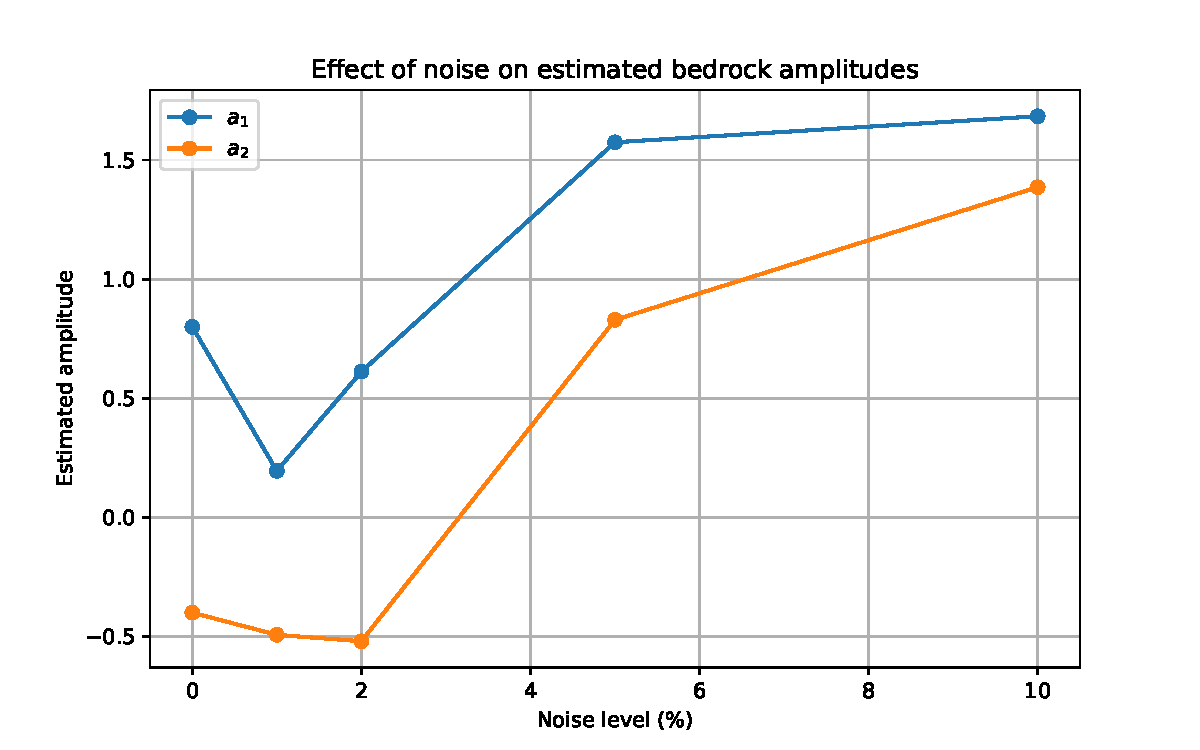
\includegraphics[width=0.75\linewidth]{Noise_Amplitudes.pdf}
    \caption{Effect of increasing measurement noise on the estimated
    bedrock amplitudes using the direct inverse method}
    \label{fig:placeholder}
\end{figure}

\section{Conclusion}

In this project, an inverse model was developed to estimate the bedrock
beneath an ice sheet using observed surface elevation and horizontal
surface velocity. The surface gradient was first calculated using finite
differences, and the horizontal velocity relation from the supplied ice
model was rearranged to estimate the ice thickness. The bedrock was then
reconstructed from the relationship $b=h-H$.

The reconstructed bedrock was fitted using the prescribed two-bump
bedrock model. The resulting amplitudes for the noise-free data were

\begin{equation}
a_1 \approx 0.8,
\qquad
a_2 \approx -0.4.
\end{equation}

These amplitudes were then used in the forward model, which was run for
200 years to demonstrate the behaviour of the ice sheet using the
inferred bedrock.

The sensitivity of the inverse model to measurement noise was also
investigated. Noise levels of $0\%$, $1\%$, $2\%$, $5\%$, and $10\%$ were
tested using the same inverse method and the same underlying random
noise pattern. The results showed that the estimated amplitudes are
sensitive to measurement noise, can reduce the accuracy of the reconstructed bedrock. The changes were not monotonic, but the
estimates became substantially different from the noise-free values at
higher noise levels. In particular, the estimated value of $a_2$ changed
sign between the $2\%$ and $5\%$ noise cases.

Overall, the results demonstrate that the direct inverse method can
recover the prescribed two-bump bedrock parameters from the
noise-free observations, but that the accuracy of the reconstructed
bedrock is strongly affected by noise in the observations. This
highlights the sensitivity of inverse modelling to measurement errors,
particularly because the surface gradient is calculated directly from
the observed surface elevation.



\end{document}
